% Capítulo 10: filtrar, transformar e reduzir em sequência (soma dos quadrados dos pares).
\documentclass[border=4pt]{standalone}
\usepackage[utf8]{inputenc}
\usepackage[T1]{fontenc}
% Estilo comum das figuras de vetores (capítulo 8).
\usepackage{tikz}
\usetikzlibrary{arrows.meta, positioning, calc, decorations.pathreplacing}
\definecolor{navy}{RGB}{23,45,80}
\definecolor{laranja}{RGB}{250,110,29}
\definecolor{cinzalogo}{RGB}{107,114,126}
\definecolor{azul}{RGB}{205,222,247}
\tikzset{
  casa/.style={draw=navy, line width=0.9pt, minimum width=8mm, minimum height=7mm,
               inner sep=0pt, font=\sffamily\small},
  pronta/.style={casa, fill=azul},
  parte/.style={casa, fill=laranja!12},
  marcada/.style={casa, fill=laranja!45, draw=laranja},
  fora/.style={casa, draw=cinzalogo!60, dashed, fill=white, text=cinzalogo!60},
  indice/.style={font=\sffamily\scriptsize, text=cinzalogo},
  explica/.style={font=\sffamily\small, text=navy, anchor=east},
  legenda/.style={font=\sffamily\scriptsize, text=cinzalogo},
  rotulo/.style={font=\sffamily\small\bfseries, text=navy},
  seta/.style={-{Stealth[length=2.2mm]}, navy, line width=0.9pt},
  chave/.style={decorate, decoration={brace, amplitude=4pt, mirror}, navy, line width=0.8pt},
}
% \vetor{nome}{x}{y}{valor/estilo, valor/estilo, ...}: casas lado a lado, chamadas nome0, nome1...
\newcommand{\vetor}[4]{%
  \foreach \valor/\estilo [count=\i from 0] in {#4} {
    \node[\estilo] (#1\i) at ($(#2, #3) + (\i*0.8, 0)$) {\valor};
  }
}

\tikzset{
  etapa/.style={font=\sffamily\small\bfseries, text=laranja, anchor=west},
  funcao/.style={font=\ttfamily\small, text=navy, anchor=west},
}
\begin{document}
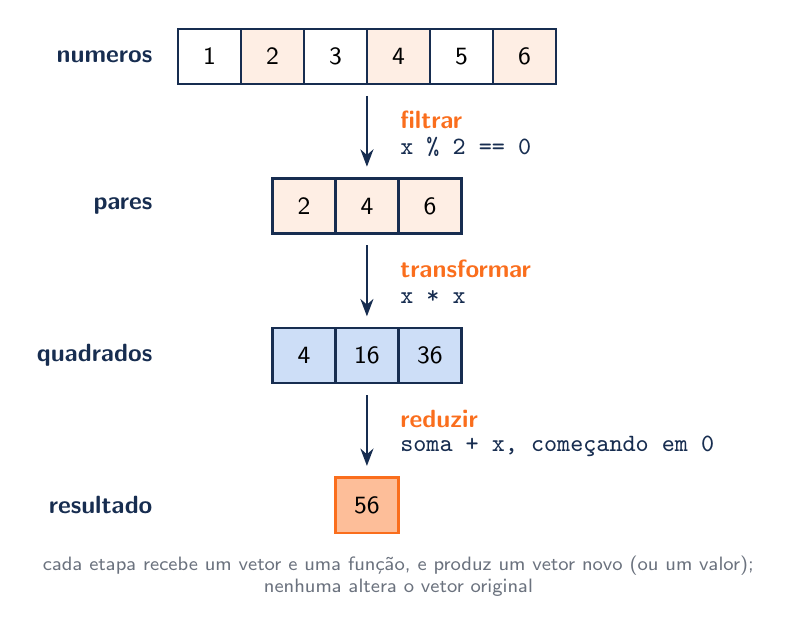
\begin{tikzpicture}
  \vetor{a}{0}{0}{1/casa, 2/parte, 3/casa, 4/parte, 5/casa, 6/parte}
  \node[rotulo, anchor=east] at (-0.6, 0) {numeros};
  \draw[seta] (2, -0.5) -- (2, -1.4);
  \node[etapa] at (2.3, -0.8) {filtrar};
  \node[funcao] at (2.3, -1.15) {x \% 2 == 0};

  \vetor{b}{1.2}{-1.9}{2/parte, 4/parte, 6/parte}
  \node[rotulo, anchor=east] at (-0.6, -1.9) {pares};
  \draw[seta] (2, -2.4) -- (2, -3.3);
  \node[etapa] at (2.3, -2.7) {transformar};
  \node[funcao] at (2.3, -3.05) {x * x};

  \vetor{c}{1.2}{-3.8}{4/pronta, 16/pronta, 36/pronta}
  \node[rotulo, anchor=east] at (-0.6, -3.8) {quadrados};
  \draw[seta] (2, -4.3) -- (2, -5.2);
  \node[etapa] at (2.3, -4.6) {reduzir};
  \node[funcao] at (2.3, -4.95) {soma + x, começando em 0};

  \node[marcada] (r) at (2, -5.7) {56};
  \node[rotulo, anchor=east] at (-0.6, -5.7) {resultado};
  \node[legenda, align=center] at (2.4, -6.6)
    {cada etapa recebe um vetor e uma função, e produz um vetor novo (ou um valor);\\
     nenhuma altera o vetor original};
\end{tikzpicture}
\end{document}
